% !TEX root = ../talk.tex

\newcommand{\varR}{2.5}
\newcommand{\varr}{1}
\newcommand{\vardi}{0.5}
\newcommand{\vardii}{0.8}
\newcommand{\varrlas}{0.4}
\newcommand{\varhlas}{0.5}

\definecolor{mycoral}{RGB}{236,27,75}
\definecolor{myorange}{RGB}{242,106,68}

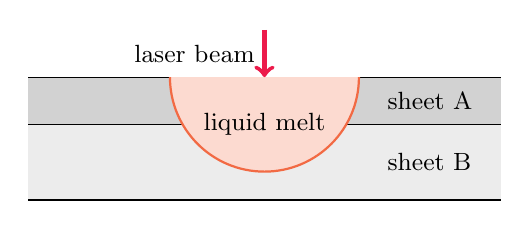
\begin{tikzpicture}[scale=1.2]

	% fillers
	\draw [draw=none, fill=gray!35] (-\varR,0) rectangle (\varR,-\vardi);
	\draw [draw=none, fill=gray!15] (-\varR,-\vardi) rectangle (\varR,-\vardi-\vardii);

	% lines
	\draw (-\varR,-\vardi) -- (\varR,-\vardi);
	\draw (-\varR,-\vardi-\vardii) -- (\varR,-\vardi-\vardii);
	\draw (-\varR,0) -- (-\varr,0);
	\draw (\varr,0) -- (\varR,0);

	\draw [myorange, thick, fill=myorange!25] (0,0) ++(180:\varr) arc (180:360:\varr);

	% laser
	\draw [->, ultra thick, color=mycoral] (0,\varhlas) -- (0,0);

	% captions
	\draw (0,.5*\varhlas) node [left] {\small laser beam};
	\draw (1.2*\varr,-.5*\vardi) node [right] {\small sheet A};
	\draw (1.2*\varr,-\vardi-.5*\vardii) node [right] {\small sheet B};
	\draw (0,-.5*\varr) node {\small liquid melt};
\end{tikzpicture}
